\chapter{流体}

\section*{A 组}
\vspace{0.3cm}
\textbf{6-1} 两端开口、向上直立的 $U$ 型试管内盛有水银. 今从试管右端缓慢注入 13.6 cm 高的水柱, 左管水银未外溢, 试求左管水银面上升的高度 $h$.


\begin{center}
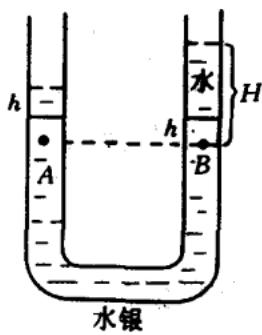
\includegraphics[width=0.15\textwidth]{figures/图6_1.jpg}
\end{center}

\vfill

\textbf{6-2} 西藏布达拉宫的海拔高度为 3756.5 $m$, 不计大气温度随高度的变化, 试求该处大气压强 $p$.


\vfill

\newpage

\textbf{6-3} 长和宽同为 $L$ 的长方容器中盛有密度为 $\rho$ 、高也为 $L$ 的液体，开始时静止在水平地面上。今使容器以恒定的加速度 $a = g / \sqrt{3}$ 水平朝右运动，如图所示。大气压强记作 $p_{0}$ ，容器中液体稳定静止后，试求液体中压强的最大值 $p_{max}$ 。

\begin{center}
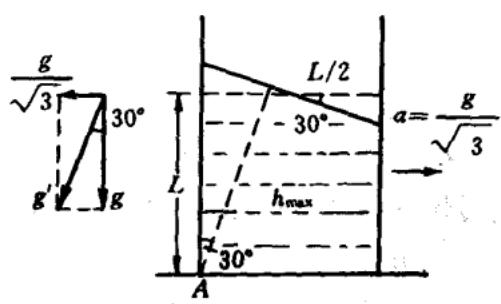
\includegraphics[width=0.35\textwidth]{figures/图6_3.jpg}
\end{center}

\vfill

\textbf{6-4} 将两个半径同为 $R=20\,cm$ 的半球壳，合成“马德堡球”，估算两侧各需施加多大的力方可将球拉成两半？


\vfill

\newpage

\textbf{6-5} 一根横截面积 $S_{1} = 5.00\mathrm{cm}^{2}$ 的细管连接在一个容器上，容器的横截面积 $S_{2} = 100\mathrm{cm}^{2}$ ，高度 $h_2 = 5.00\mathrm{cm}$ . 今将水注入，使水相对容器底部的高度 $h_1 + h_2 = 100\mathrm{cm}$ ，如图所示.

(1) 计算水对容器底部的压力值和容器内水的重力；

(2) 解释这两个值为何不同.

\begin{center}
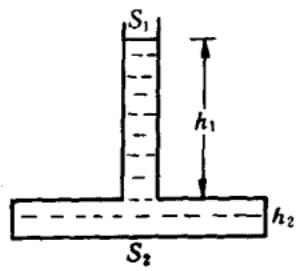
\includegraphics[width=0.2\textwidth]{figures/图6_4.jpg}
\end{center}

\vfill

\textbf{6-6} 冰的密度记为 $\rho_{1}$ , 海水密度记为 $\rho_{2}$ , 有 $\rho_{1} < \rho_{2}$ . 金字塔形 (正四棱锥) 的冰山漂浮在海水中, 平衡时塔顶离水面高度为 $h$ , 试求冰山自身高度 $H$ .


\vfill

\newpage

\textbf{6-7} 一根长为 $l$、密度为 $\rho$ 的匀质细杆，浮在密度为 $\rho_{0}$ 的液体里。杆的一端由一竖直细绳悬挂着，使该端高出液面的距离为 $d$，如图所示。

(1) 计算杆与液面的夹角 $\theta$ ;

(2) 设杆的截面积为 $S$, 计算绳中的张力 $T$.

\begin{center}
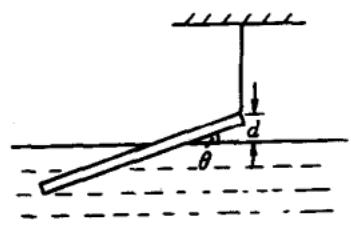
\includegraphics[width=0.2\textwidth]{figures/图6_5.jpg}
\end{center}

\vfill

\textbf{6-8} 在一截面积为 $50 \, cm^{2}$ 的水管上接有一段弯管，使管轴偏转 $75^{\circ}$ ，如图所示。设管中水的流速为 $3.0 \, m/s$ ，试求水流作用在弯管上力的方向和大小 $F$。


\begin{center}
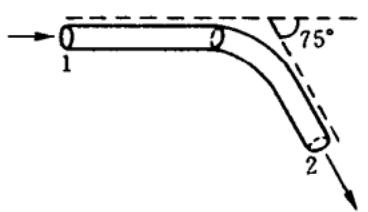
\includegraphics[width=0.2\textwidth]{figures/图6_7.jpg}
\end{center}

\vfill

\newpage

\textbf{6-9} 图 6-9 所示的直立容器盛水高度 $H$，图中 $A$, $B$ 两处容器截面积分别为 $S_{A}, S_{B}$ . 将下端 $C$ 处活塞打开后，水的流动近似处理成定常流动. 试问各在什么样的条件下，$A$, $B$ 两处压强 $p_{A}, p_{B}$ 间分别满足
\[
p _ {A} = p _ {B}, \quad p _ {A} <   p _ {B}, \quad p _ {A} > p _ {B}.
\]

\begin{center}
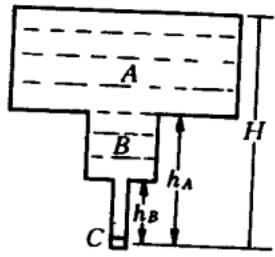
\includegraphics[width=0.2\textwidth]{figures/图6_9.jpg}
\end{center}

\vfill

\textbf{6-10} 圆桶形油箱内盛有水和石油, 水的厚度为 1 $m$, 油的厚度为 4 $m$, 石油密度为 $0.9 \times 10^{3} \, kg/m^{3}$ , 试求水从箱底小孔流出时的速度 $v$.


\vfill

\newpage

\textbf{6-11} 桶的底部有一洞,水面距桶底 30 cm. 当桶以 $120 \, m/s^{2}$ 的加速度上升时,水从洞漏出的速度多大?


\vfill

\textbf{6-12} 为了避免火车停下来加水, 可在铁轨旁设置长水槽, 从火车上垂挂一根弯水管于水槽中, 使水沿管上升流入火车的水箱, 如图所示. 如果水箱与水槽的高度差为 $h = 3.5 \mathrm{~m}$ , 那么火车的速度至少达多大才能使水流入箱中? 若火车走了 $L = 1.00 \mathrm{~km}$ 的路程要使水箱得到体积为 $V=3.00\ m^{3}$ 的水，已知水管直径 d=10 cm，试问火车速度为多大？


\begin{center}
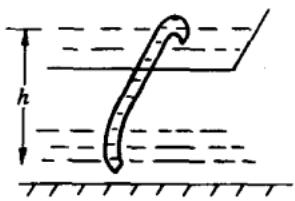
\includegraphics[width=0.2\textwidth]{figures/图6_10.jpg}
\end{center}

\vfill

\newpage

\textbf{6-13} 匀速地将水注入大水盆内, 注入的流量 $Q_{V}=150\ cm^{3}/s$ , 盆底有一小孔, 面积为 $0.50\ cm^{2}$ , 求稳定时水面将在盆中保持的高度 $h$.

\vfill

\textbf{6-14} 在一直径很大的圆柱形水桶壁的近底部处有一直径为 0.04 $m$ 的小孔，桶内水的深度为 1.60 $m$. 求：

(1) 此时从小孔中流出的体积流量 $Q_{1}$ ;

(2) 若小孔为薄壁圆孔, 收缩系数为 61\%, 实际的体积流量 $Q_{2}$ .

\vfill

\newpage

\textbf{6-15} 一倒立的圆锥形容器, 高为 $H$, 底面半径为 $R$. 容器内装满水, 下方锥顶角处有一面积为 $S$ 的小孔, 水从小孔中流出, 试求水面下降到 H/2 高度时所需的时间 $t$.


\vfill

\textbf{6-16} 图6-11中的水平圆柱形桶内盛水高度 $h_1 = 50\mathrm{cm}$ , 插入的细弯管称为虹吸管, 下端 $C$ 在桶底下方 $h_2 = 40\mathrm{cm}$ 处, 虹吸管侧面与另一开口的细弯管连通. 开始时虹吸管内已充满水, 而后将 $C$ 处小活塞打开, 设很短时间内右侧弯管水面 $Q_0$ 降落到某一个近似稳定的位置 $Q$ . 先求 $C$ 处水流速度 $v_C$ , 再确定 $Q$ 与 $C$ 之间的高度差 $h_{QC}$ .

\begin{center}
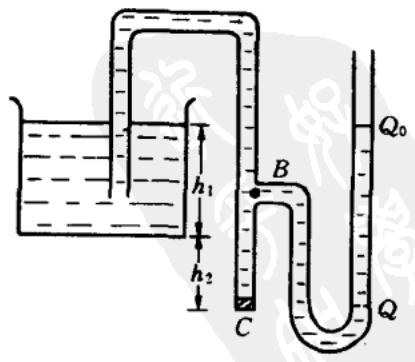
\includegraphics[width=0.3\textwidth]{figures/图6_11.jpg}
\end{center}

\vfill

\newpage

\textbf{6-17} 将犬的一根大动脉中流动的血液接到一支两直管型文丘里流量计上. 流量计宽段面积 $S_{1}=0.08\ cm^{2}$ ，它等于这根动脉的横截面积，细段面积 $S_{2}=0.04\ cm^{2}$ ，流量计中显示的压强差为 25 Pa. 已知血液密度 $\rho=1060\ kg/m^{3}$ ，试求动脉血液的体积流量 $Q_{V}$ .


\vfill

\textbf{6-18} 一喷泉竖直喷出高 $H$ 的水流, 喷泉的喷嘴具有上细下粗的截锥形状, 上截面的直径为 $d$, 下截面的直径为 $D$, 喷嘴高为 $h$. 设大气压强为 $p_{0}$ , 试求:

(1) 水的体积流量 $Q_{v}$ ;

(2) 喷嘴下截面处水的压强 $p_{D}$ .

\vfill

\newpage

\textbf{6-19} 在直径为305 mm的输油管内, 安装了一个开口面积为原面积1/5的隔片, 管中的石油体积流量为 $70 \times 10^{-3} \, m^{3}/s$ , 其运动黏度 $\eta/\rho = 1.0 \times 10^{-4} \, m^{2}/s$ . 试问石油经过隔片时, 是否变为湍流?


\vfill

\textbf{6-20} 血液密度与水的密度相近, 黏度 $\eta=4.0\times10^{-3}$ Pa·s. 犬的一根大动脉内半径 r=4 mm, 平均血液流速 $\bar{v}=40$ m/s, 试问其内的血液流动是层流还是湍流？

\vfill

\newpage

\textbf{6-21} 油泵将黏度 $\eta=0.30\ Pa\cdot s$ 的油，经过半径 $R=0.10\ m$ 的水平钢管运送到 $l=100\ m$ 的远处。已知体积流量 $Q_{V}=0.05\ m^{3}/s$ ，试求油泵显示的管道两端间压强差 $\Delta p$ 和油泵消耗的功率 $P$。

\vfill

\textbf{6-22} 密度为 $\rho$ 的黏性液体, 因重力作用在半径为 $R$ 的竖直圆管道内向下作定常流动. 已测得管道的体积流量为 $Q_{v}$ , 试求液体的黏度 $\eta$ .

\vfill

\newpage

\textbf{6-23} 已知空气的密度 $\rho_{A}=1.3\ kg/m^{3}$ ，黏度 $\eta=1.81\times10^{-5}\ Pa\cdot s$ ，试分别计算半径 $r_{1}=1.0\times10^{-3}\ mm$ 和 $r_{2}=5.0\times10^{-2}\ mm$ 的雨滴下落的终极速度 $v_{e1}$ 和 $v_{e2}$ .

\vfill

\textbf{6-24} 密度为 $2.56 \mathrm{~g} / \mathrm{cm}^{3}$ 、半径为 $3.0 \mathrm{~mm}$ 的玻璃球，在一盛甘油的筒中从静止下落。已知甘油密度为 $1.26 \mathrm{~g} / \mathrm{cm}^{3}$ ，测得玻璃球最终恒定的速度为 $3.1 \mathrm{~cm} / \mathrm{s}$ ，试求甘油黏度 $\eta$ 和小球下落过程中加速度恰为 $g / 2$ 时的速度 $v$ 。

\vfill

\newpage

\textbf{6-25} 半径为0.10 cm的小空气泡在密度为 $0.72 \times 10^{3} \, kg/m^{3}$ 、黏度为0.11 Pa·s的液体中上升，求其上升的终极速度.

\vfill

\textbf{6-26} 半径 $r = 0.01 \mathrm{~mm}$ 的水滴，在速度为 $v_{0} = 2 \mathrm{~cm} / \mathrm{s}$ 的上升气流中是否会朝地面回落？已知空气的黏度 $\eta = 1.8 \times 10^{-5} \mathrm{~Pa} \cdot \mathrm{s}$ .

\vfill

\newpage

\section*{B 组}
\vspace{0.3cm}
\textbf{6-27} 已知流体的二维速度场分布为
\[
v _ {x} = \frac {- c y}{x ^ {2} + y ^ {2}}, \quad v _ {y} = \frac {c x}{x ^ {2} + y ^ {2}}.
\]

(1) 导出流体的二维加速度场分布；

(2) 画出二维流线；

(3) 画出流体质元的二维迹线, 据此导出质元在 $(x, y)$ 处的加速度分量 $a_x, a_y$ .

\vfill

\textbf{6-28} 灭火器唧筒向上喷水, 喷口截面 $1.5 \mathrm{~cm}^{2}$ , 喷水的体积流量为 $1 \mathrm{dm}^{3} / \mathrm{s}$ . 有同学估算水柱在 $2 \mathrm{~m}$ 高处的截面积为 $4.35 \mathrm{~cm}^{2}$ , 你认为他是怎样得到这一结果的? 你对他的估算方法有何评论?

\vfill

\newpage

\textbf{6-29} 一个有旋转对称表面的水壶,其对称轴沿竖直方向,在正中间的壶底开一个半径为 $r_{0}$ 的小孔，为使液体从底部小孔流出的过程中壶中液面下降的速率保持不变，试求壶的表面形状。（古代用此漏壶计时。）

\vfill

\textbf{6-30} 宽度同为 $L$ 的两块无穷大平行平板相距 2H，黏度为 $\eta$ 的流体在板间从左端 1 向右端 2 作定常流动，两端的外加压强分别为 $p_{1}, p_{2}$ . 设流体与板接触处流速为零，以两板间的中央位置为原点设置图 6-14 所示的 $x$ 轴，略去流体重力影响，试求流速分布 $v = v(x)$ .

\begin{center}
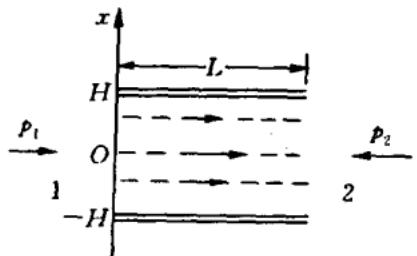
\includegraphics[width=0.3\textwidth]{figures/图_6_14.jpg}
\end{center}

\vfill

\newpage

\textbf{6-31} 半径分别为 $R_{1}, R_{2} > R_{1}$ 的长圆柱形薄筒竖直同轴放置，两筒间充满密度为 $\rho$ 常量的液体。今使内筒以恒定的角速度 $\omega_{0}$ 绕轴旋转，外筒静止，因液体的黏性，与内筒接触的液体部位均随内筒一起旋转，与外筒接触的液体部位均随外筒一起静止。设液体黏度处处相同，流体已形成稳定的层流结构，密度 $\rho$ 不变，不计重力影响。

(1) 试求流体绕轴旋转角速度 $\omega$ 随径矢 $r$ 的分布函数；

(2) 已知流体中 $r = R_{1}$ 处的压强为 $p_{0}$ ，试求液体压强 $p$ 随 $r$ 的分布函数.


\vfill
